\section{Literature Review}
\subsection{Introduction}
Fluid flow experiments involve determination of the flow velocity, the mass flow rate or volumetric flow rate. These experiments are used to familiarize the students with typical methods of flow measurement of an incompressible fluid and, at the same time demonstrate applications of the Bernoulli's equation. Thus, these experimental investigations require the application of measuring techniques to yield quantitative information on the relationship between pressure, temperature and local flow velocities.
\par
The synthetic hydro-experimental machine employs the use of the venture and the orifice meter in determining these fluid properties specifically the coefficient of discharge. It involves determining the relationship between a flowing fluid through a valve, the weight and temperature of the collected discharge. The machine comprises of four main parts; the diverter, gate valve, weight and temperature measurement unit. The measurement involves four main processes, discharge collection, diversion, weight and temperature measurement. 
\subsubsection{Gate Valve }
\par
The valve is attached at the end of the pipeline immediately after the venture and the orifice meter. It is used in flow rate control by either increasing or reducing the aperture at which the fluid flows. The experiment is conducted in several steps which is determined by opening and closing of the valve. At the start of the experiment, the valve is initially closed hence no fluid is collected. Depending on the required number of steps, the valve is then opened in small steps allowing the discharge to be collected for purposes of weight and temperature measurement.
\subsubsection{Diverter }
\par
After each step of the experiment, the collected fluid flows into the weight measurement unit through the help of a diverter. The diverter is used to direct the collected discharge into the weight measurement unit which is located at the periphery of the rig to avoid flowing back into the reservoir. The diverter is a mechanical device that is moved by hand.
\subsubsection{Temperature measurement unit }
\par
 The temperature of the collected discharge is measured immediately after the fluid flows through the gate valve by use of a thermometer. This is to minimize the environmental effects, for instance the effects of the metallic diverters which would otherwise compromise on the temperature readings. The readings are measured and recorded after each step of the experiment.
\subsubsection{Pressure measurement }
\par
The differential manometers are attached just before and after both the venture and the orifice and is used to determine the pressure of the flowing fluid. These manometric readings are recorded after each and every step of the experiment.
\subsubsection{Weight measurement unit }
\par
The final part involves measuring the weight of the collected discharge. This is done by use of a measuring scale with loads attached to it. The above measurements are then used to establish the coefficient of discharge of the fluid.
\subsection{Existing Technologies}
Some advanced and even rudimentary technologies have been used in place of the Synthetic Hydro-Experimental machine for the determination of fluid flow properties. The technologies include :   
\subsubsection{Computational Fluid Dynamics}
Computational fluid dynamics(CFD) is a powerful modelling and analysis technique that utilizes finite difference techniques to solve highly non-linear differential equation of pressure, energy, relative humidity, air temperature and velocity \cite{raman2018review}. It can be used to model fluid flow in flow measurement devices.
\par
Tukimin et al \cite{tukimin2016cfd} in their study  conducted a CFD analysis using an Single Kernel Estimate (SKE) turbulence model to determine the coefficient of discharge of a Venturi tube, and finally compared the results to those obtained from a physical experimental setup. The test loop shown in figure \ref{fig:test_loop_rig} was used both in a physical setup and a CFD model. 

\begin{figure}[ht]
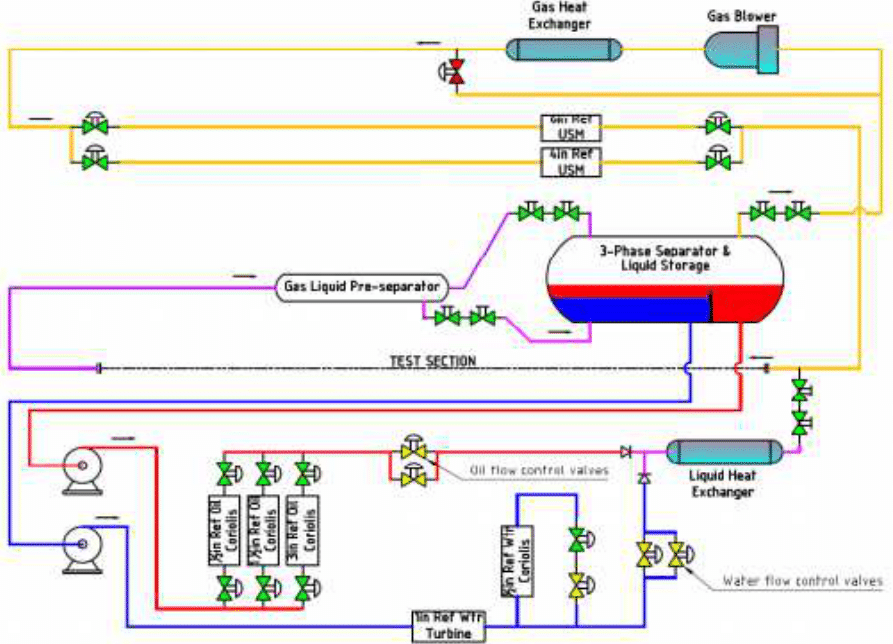
\includegraphics[width=0.9\linewidth]{Figures/test_loop.png}
\centering
\caption[Test loop schematic]{ Test loop schematic by Tukimin et al \cite{tukimin2016cfd}}
\label{fig:test_loop_rig}
\end{figure}

They designed a CFD model using the ANSYS Design Modeller software. The model consists of a Venturi tube, designed according to the standards ISO 5167:2003 \cite{carello2013flow}, and a liquid and gas system. They did a physical experiment using the same test matrix used in the numerical simulation model. Finally, they computed the coefficient of discharge of the venturi using equationt \ref{eq:2}.  

\begin{equation}
C d=\frac{4 m \sqrt{1-\beta^{4}}}{\pi \varepsilon d^{2} \sqrt{200000 D p_{1} \rho_{1}}}
\label{eq:2}
\end{equation}

\begin{table}[!t]
  \begin{center}
    \leavevmode
    \hangcaption{ Calculated $C_{d}$}   
     \begin{tabular}{rlc}\hline
      Venturi under Test & Average Discharge Coefficient &  Average Discharge Coefficient \\ \hline
       & From experiment &  From CFD post \\ \hline
      Venturi 1 & 0.99366 &  0.984347 \\ \hline
    \end{tabular}
    \label{tab:cd}
  \end{center}
\end{table}
The results obtained in \ref{tab:cd} showed a difference of less than $1 \%$ between the $C_{d}$ obtained from the two setups.
\par
Tamhankar et al \cite{tamhankar2014experimental} also did a similar experiment using a CFD model designed in ANSYS Fluent 13.0 utilizing a Realizable k-$\epsilon$ turbulence model which is superior to a Standard k-$\epsilon$ turbulence model and compared the results to those obtained from an experimental setup show in figure \ref{fig:exp}. 


\begin{figure}[ht]
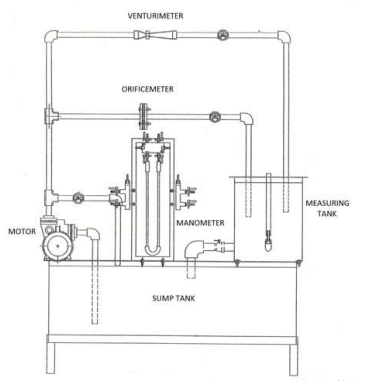
\includegraphics{Figures/exp.png}
\centering
\caption[Experimental setup ]{ Experimental setup by Tamhankar et al \cite{tamhankar2014experimental}}
\label{fig:exp}
\end{figure}

Table \ref{tab:results} shows the results obtained from the study
\begin{table}[!t]
    \centering
    \hangcaption{Results}
    \begin{tabular}{|c|c|c|}
        \hline \text { Reading No. } & \text { Experiment } & \text { CFD analysis } \\
        \hline 1 & 0.9724 & 0.9619 \\
        \hline 2 & 0.9592 & 0.9689 \\
        \hline 3 & 0.9779 & 0.9692 \\
        \hline
    \end{tabular}
    \label{tab:results}
\end{table}

The study concluded that difference in values of the coefficient of discharge obtained from the model and those obtained from the experimental setup was less than $ 5 \%$ .
\subsubsection{Analytical Predictions}
This technique utilizes the Bernoulli's equation to establish an analytical correlation between the fluid flow and the coefficient of discharge of the Venturi meter. 

\begin{figure}
    \centering
    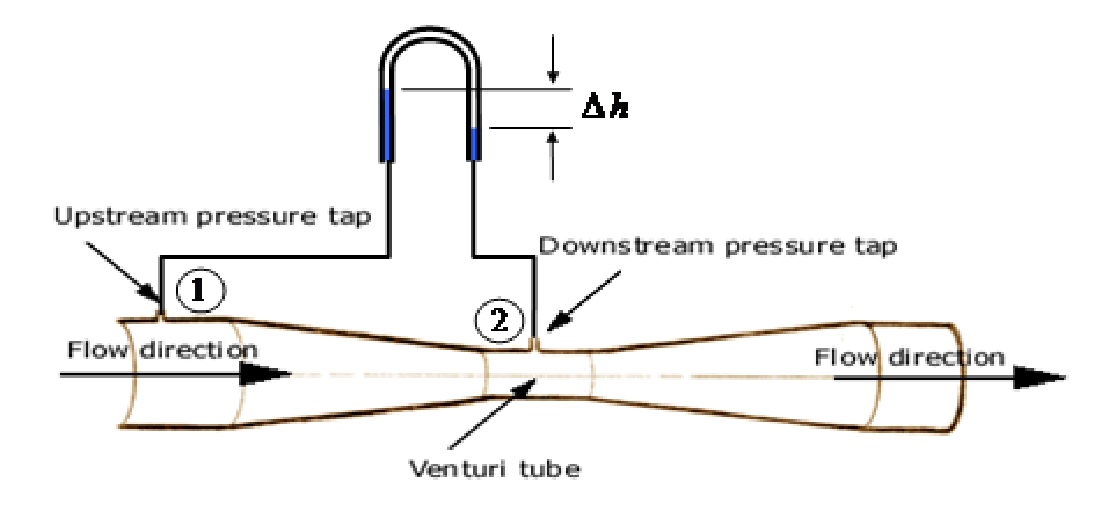
\includegraphics[width=0.6\linewidth]{Figures/venturi.png}
    \caption[Venturi Meter]{Venturi meter \cite{venturi_meter}}
    \label{fig:venturi}
\end{figure}

Figure \ref{fig:venturi} shows the Venturi meter. Assuming the flow is ideal and applying the Bernoulli's equation before and after the contraction, 

\begin{equation}
\begin{aligned}
&\frac{p_{1}}{\rho g}+\frac{v_{1}^{2}}{2 g}+z_{1}=\frac{p_{2}}{\rho g}+\frac{v_{2}^{2}}{2 g}+z_{2} \\
&\text { But } Z_{1}=Z_{2}, \\
&\frac{\left(p_{1}-p_{2}\right)}{\rho}=\frac{\left(v_{2}^{2}-v_{1}^{2}\right)}{2} \\
&\frac{\left(p_{1}-p_{2}\right)}{\rho}=\frac{v_{2}^{2}}{2}\left(1-\frac{A_{2}^{2}}{A_{1}^{2}}\right) \\
&\frac{\Delta p}{\rho}=\frac{v_{2}^{2}}{2}\left(1-\beta^{4}\right) \\
&v_{2}=\frac{1}{\sqrt{1-\beta^{4}}} \sqrt{\frac{2 \Delta p}{\rho}}
\end{aligned}
\label{eq:bernoulli_der}
\end{equation}

Applying the continuity equation to the result of the derivation in \ref{eq:bernoulli_der},
\begin{equation}
\begin{aligned}
&Q_{t h}=A_{1} v_{1}=A_{2} v_{2} \\
&Q_{t h}=A_{2} v_{2}=\frac{1}{\sqrt{1-\beta^{4}}} \frac{\pi d^{2}}{4} \sqrt{\frac{2 \Delta p}{\rho}}
\end{aligned}
\label{eq:mass_flow_rate}
\end{equation}
Equation \ref{eq:mass_flow_rate} of theoretical flow rate is based on the assumption that the flow is steady, incompressible, inviscid, irrotational, no losses and the velocities $V_{1}$ and  $V_{2}$ are constant across the cross section \cite{arun2015prediction}. 

\begin{equation}
\mathrm{Q}_{\mathrm{act}}=\frac{\mathrm{C}_{\mathrm{d}_{\mathrm{st}} \mathrm{d}}}{\sqrt{1-\beta^{4}}} \frac{\pi \mathrm{d}^{2}}{4} \sqrt{\frac{2 \Delta \mathrm{p}}{\rho}}
\end{equation}
The frictional and viscous losses in a laminar flow can be estimated by the Darcy's law
\begin{equation}
\mathrm{H}_{\mathrm{L}}=\frac{(\Delta \mathrm{p})_{\text {viscous }}}{\rho \mathrm{g}}=\mathrm{f} \frac{\mathrm{v}^{2}}{2 \mathrm{~g}} \frac{\mathrm{D}}{\mathrm{D}}
\end{equation}
where 'f' is the friction factor.
\par
Coefficient of discharge equation \ref{eq:cd2} where for laminar flow, 'f' is given by equation \ref{eq:f} . This equation is derived from both the Darcy's law equation and the theoretical flow rate equation \ref{eq:mass_flow_rate}.
\begin{equation}
f=\frac{64}{R_{e d}}
\label{eq:f}
\end{equation}


\begin{equation}
C_{\mathrm{d}}=0.995 \sqrt{\frac{1}{(1+3 f)}}
\label{eq:cd2}
\end{equation}

\par
Arun et al \cite{arun2015prediction} did  a comparision of the $C_{d}$ obtained by this method and that obtained from a CFD simulation. The study concluded that the results from the two methods had an uncertainty of $0.9\%$.
\subsection{Related Works}
Discharge collection techniques have been developed for various applications. Some of these applications are related to the discharge collection unit used in the Synthetic Hydro-Experimental machine.

\subsubsection{Electromagnetic activation}
Angelo et al \cite{odetti2019design} implemented this technique in the design and testing of an Modular Automatic Water Sampler(MAWS). They designed MAWS and mounted them on unmanned marine vehicle with the aim of collecting water samples for scientific campaigns in front of polar tidewater glaciers. Their main design considerations was the response time of the stopper since the MAWS were operated under water and at the risk of damage by glaciers. The actuation unit of the sampler is shown in figure \ref{fig:stopper}. 

\begin{figure}
    \centering
    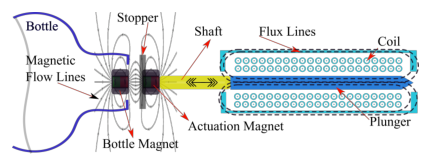
\includegraphics{Figures/stopper.png}
    \caption[Sampler actuation mechanism]{Sampler actuation mechanism \cite{odetti2019design}}
    \label{fig:stopper}
\end{figure}

When the coil in the solenoid is crossed by a current a strong magnetic field is generated that attracts the ferromagnetic plunger connected to the sealing stopper and opens the bottle allowing water to flow into the bottle's neck. As the current stops the two permanent magnets attract each other and the stopper seals the bottle \cite{odetti2019design}.

\subsubsection{Pneumatic Control}
Pneumatic actuators utilizes the power of compressed air to impart motion on objects. Sangmin, and Joonwon \cite{lee2009development} did a design of cartridge-type pneumatic dispenser with a back flow stopper. The system used a membrane covering a discharge hole. The membrane was opened and closed using negative and positive pneumatic pressure respectively as shown in figure \ref{fig:dispensing_mechanisml}. 

\begin{figure}
    \centering
    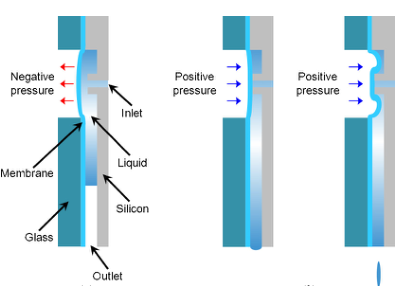
\includegraphics{Figures/dispensing_mechanism.png}
    \caption[Dispensing mechanism]{Dispensing mechanism \cite{lee2009development}}
    \label{fig:dispensing_mechanisml}
\end{figure}

The application was able to do precise dispensation of 100nL to 400nL droplets.

\subsection{Summary}

Every fluid flow experiment done on the Synthetic Hydro-Experimental machine involves the collection of discharge and the measurement of its properties. The most common experiment is the determination of the coefficient of discharge  of the Venturi and the Orifice. In this literature, other techniques such as CFD and analytical methods have been found to be effective as alternatives to this machine. These techniques have been proven to produce results with a difference of less than $1\%$  from the experimental results obtained from a physical setup. Such results can also be obtained from the fluids rig currently used in JKUAT by automating the discharge collection unit. With regard to this, the literature has also covered discharge collection techniques that have proven to be effective in other applications and can be adapted for this automation. This techniques include the application of pneumatics and electromagnetism. 

\subsection{Gap analysis}
\begin{enumerate}
    \item The use of the CFD method or the analytical method  undermines the credibility of the fluid flow experiments. This two techniques are rather used for the design of fluid flow measuring devices.
    \item CFD method can also be very resource intensive in terms of compute resources. Softwares used for this method requires a hefty license fee.
    \item The application of the analytical method involves tedious calculations and several assumptions which can produce untrustworthy results.
    \item The use of the Synthetic Hydro-Experimental machine with a manual discharge collection unit often produce results with huge error margins.  
\end{enumerate}

This project proposal is entirely focused on addressing gap number four with the application of techniques such as pneumatics or electromagnetism. This closes in the technological gap with the use of CFD, and simplify the use of analytical methods by providing data for the computation of fluid flow properties.    





